% DFA tikz examples
% A lot of the technique to making them look good is proper position, which
% admittedly can take some practice
\documentclass[12pt]{article} % My goto default. Pretty standard

\usepackage{tikz} % Package
\usetikzlibrary{automata,positioning} % For automata

% INDISPENSABLE for margins
\usepackage[margin=1in]{geometry}

\title{DFA Examples Using TikZ}
\author{github.com/adelman}
\date{}

\begin{document}
\maketitle

\paragraph{Example 1:\\}
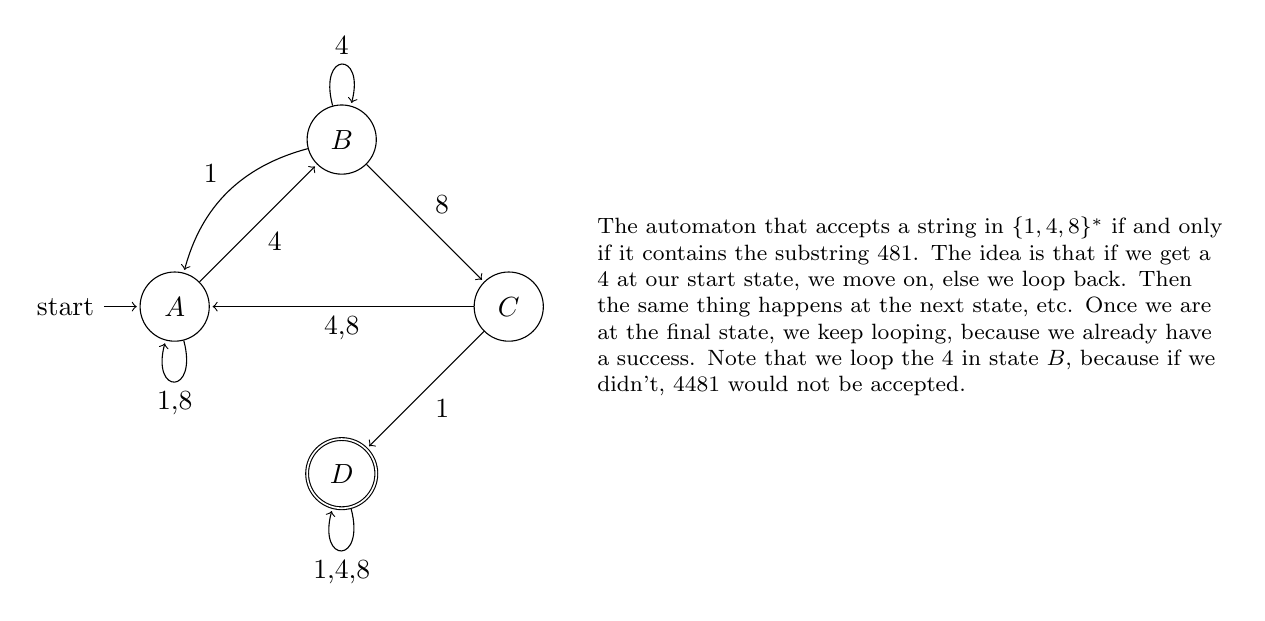
\begin{tikzpicture}[shorten >=1pt,node distance=3cm,on grid,auto] 
    % For nodes, you define their type, then the label, then display name
    \node[state, initial]   (A)   {$A$};
    \node[state]            (B) [above right=of A] {$B$};
    \node[state]            (C) [below right=of B] {$C$};
    \node[state,accepting]  (D) [below right=of A] {$D$};
    \path[->]
    (A) edge [loop below] node {1,8} ()
        edge node [swap] {4} (B)
    (B) edge [bend right] node [swap] {1} (A)
        edge [loop above] node {4} ()
        edge node {8} (C)
    (C) edge node {4,8} (A)
        edge node {1} (D)
    (D) edge [loop below] node {1,4,8} ();
    \node [right=1cm,text width=8cm,font=\footnotesize] at (C) { The automaton
    that accepts a string in $\{1,4,8\}^*$ if and only if it contains the
    substring $481$. The idea is that if we get a $4$ at our start state, we
    move on, else we loop back. Then the same thing happens at the next state,
    etc.  Once we are at the final state, we keep looping, because we already
    have a success. Note that we loop the 4 in state $B$, because if we didn't,
    $4481$ would not be accepted. };
\end{tikzpicture}

\paragraph{Example 2:\\}

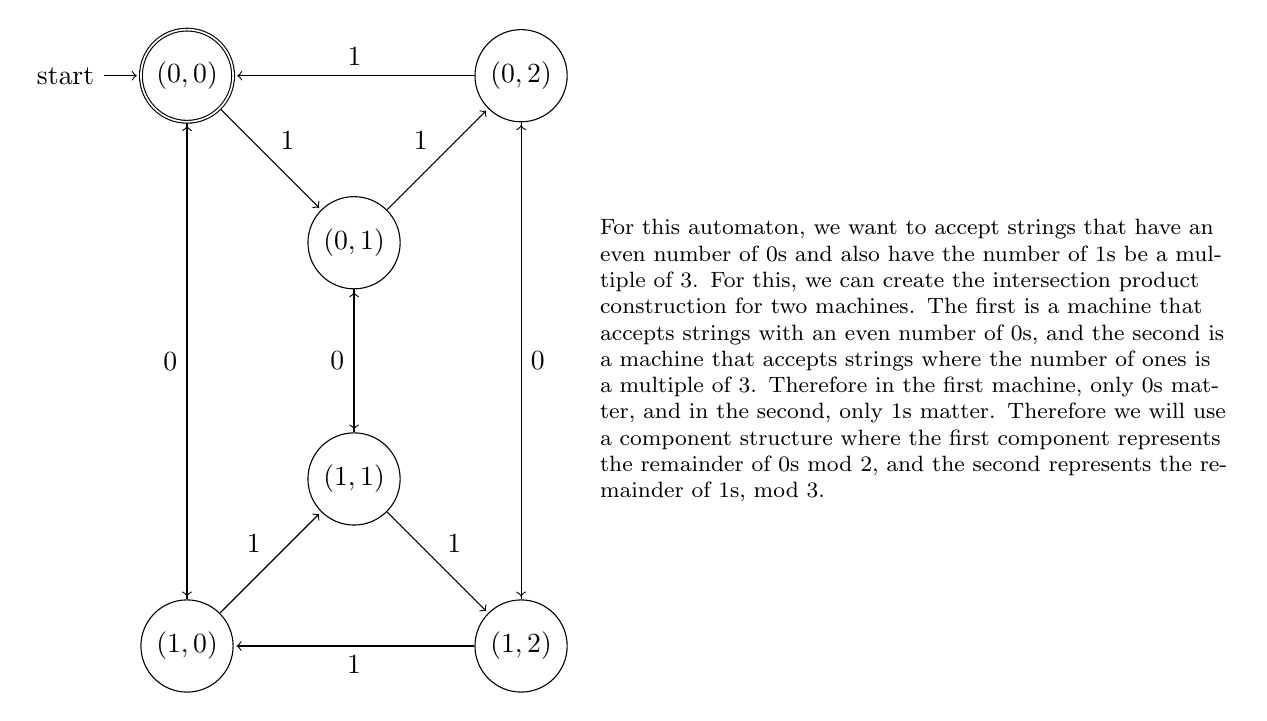
\begin{tikzpicture}[shorten >=1pt,node distance=3cm,on grid,auto] 
    \node[state,initial,accepting]  (00)    {$(0,0)$}; 
    \node[state] (01) [below right=of 00]   {$(0,1)$};
    \node[state] (02) [above right=of 01]         {$(0,2)$};
    \node[state] (11) [below=of 01]    {$(1,1)$};    
    \node[state] (12) [below right=of 11]   {$(1,2)$};
    \node[state] (10) [below left=of 11]          {$(1,0)$};

    \path[->]
    (00) edge node {} (10)
         edge node {1} (01)
    (01) edge node {} (11)
         edge node {1} (02)
    (02) edge node {0} (12)
         edge node [swap] {1} (00)
    (10) edge node {0} (00)
         edge node {1} (11)
    (11) edge node {0} (01)
         edge node {1} (12)
    (12) edge node {} (02)
         edge node {1} (10);

    \node [right=3cm,text width=8cm,font=\footnotesize,
    yshift=1.5cm] at (11) { 
    For this automaton, we want to accept strings that have an even number
    of 0s and also have the number of 1s be a multiple of 3. For this, we
    can create the intersection product construction for two machines. The
    first is a machine that accepts strings with an even number of 0s, and
    the second is a machine that accepts strings where the number of ones is
    a multiple of 3. Therefore in the first machine, only 0s matter, and in
    the second, only 1s matter.  Therefore we will use a component structure
    where the first component represents the remainder of 0s mod 2, and the
    second represents the remainder of 1s, mod 3.};

\end{tikzpicture}

\paragraph{Example 3:\\}
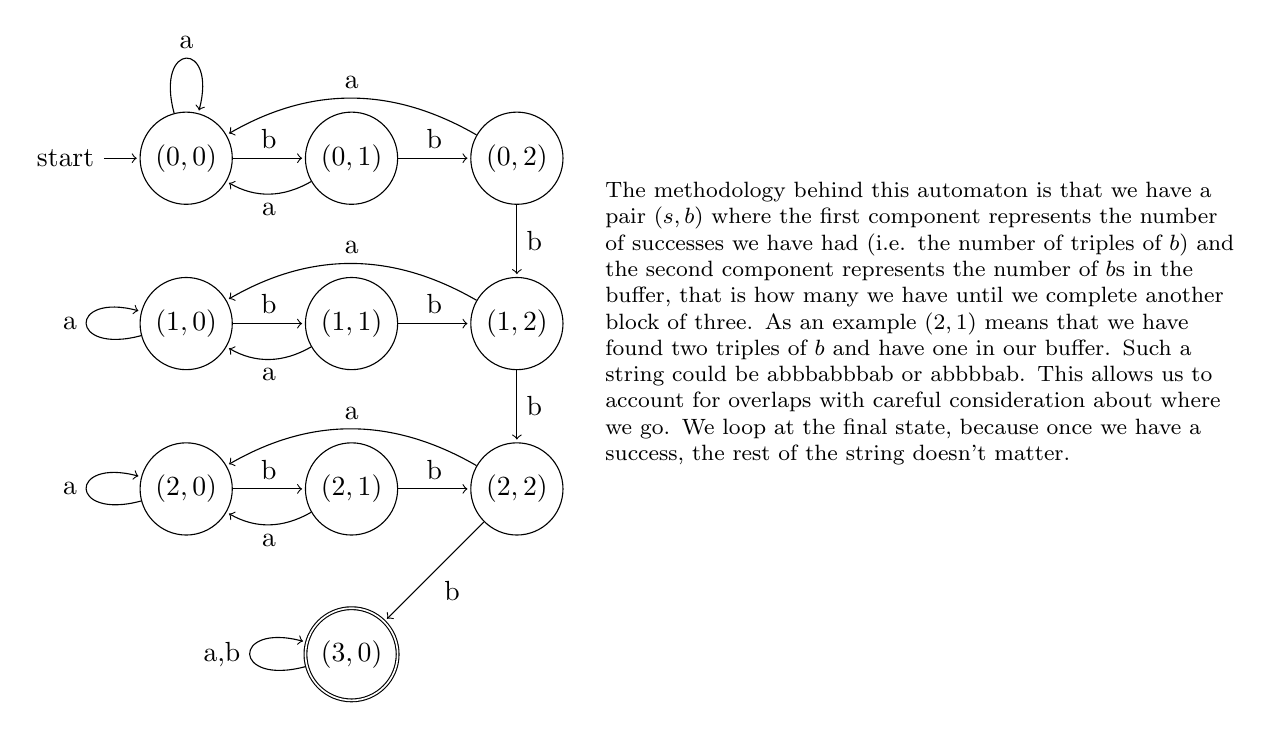
\begin{tikzpicture}[shorten >=1pt,node distance=2.1cm,on grid,auto] 
    \node[state,initial]    (00)               {$(0,0)$};
    \node[state]            (01) [right=of 00] {$(0,1)$};
    \node[state]            (02) [right=of 01] {$(0,2)$};
    \node[state]            (10) [below=of 00] {$(1,0)$};
    \node[state]            (11) [right=of 10] {$(1,1)$};
    \node[state]            (12) [right=of 11] {$(1,2)$};
    \node[state]            (20) [below=of 10] {$(2,0)$};
    \node[state]            (21) [right=of 20] {$(2,1)$};
    \node[state]            (22) [right=of 21] {$(2,2)$};
    \node[state,accepting]  (30) [below=of 21] {$(3,0)$};
    \path[->]
    (00) edge [loop above] node {a} ()
         edge node {b} (01)
    (01) edge [bend left] node {a} (00)
         edge node {b} (02)
    (02) edge [bend right] node [swap] {a} (00)
         edge node {b} (12)

    (10) edge [loop left] node {a} ()
         edge node {b} (11)
    (11) edge [bend left] node {a} (10)
         edge node {b} (12)
    (12) edge [bend right] node [swap] {a} (10)
         edge node {b} (22)

    (20) edge [loop left] node {a} ()
         edge node {b} (21)
    (21) edge [bend left] node {a} (20)
         edge node {b} (22)
    (22) edge [bend right] node [swap] {a} (20)
         edge node {b} (30)

    (30) edge [loop left] node {a,b} ();


    \node [right=1cm,text width=8cm,font=\footnotesize] at (12) { The
    methodology behind this automaton is that we have a pair $(s,b)$ where the
    first component represents the number of successes we have had (i.e. the
    number of triples of $b$) and the second component represents the number of
    $b$s in the buffer, that is how many we have until we complete another block
    of three. As an example $(2,1)$ means that we have found two triples of $b$
    and have one in our buffer. Such a string could be abbbabbbab or abbbbab.
    This allows us to account for overlaps with careful consideration about
    where we go. We loop at the final state, because once we have a success, the
    rest of the string doesn't matter.};
\end{tikzpicture}




\end{document}
